% Chapter gbm: Geometric Brownian motion and the Chebyshev bound. Chapter title for the splitter: "The primes as a portfolio of calls". Source: misc/reviews/nick-gbm-chebyshev/source/gbm_chebyshev_for_vadim/chapter_gbm_chebyshev.tex (lines 1 to 503 and 715 to 797; the completeness section 504 to 714 is a separate file, Section gbm:sec:complete), referee reports misc/research/directions/opus/vol3/GBM.md (M1 to M11) and misc/research/directions/astra/GBM/report.md, recomputation misc/vol3/verify/GBM/gbm.md.
\label{gbm:ch:main}
This chapter takes the one feature that distinguishes the inequality (M) of the preceding chapters from a general explicit formula, a nonnegative weight on ramps, and follows it as far as probability goes. The statistic of (M) is a sum of ramps $(x/n-1)_+$ with nonnegative weights, so it is convex in $x$. The ramp is the Green function of geometric Brownian motion, the statistic evaluated along the motion is a submartingale whose compensator is local time at the prime powers, and its mean is the price of Black and Scholes of a portfolio of calls struck at the prime powers. That price has an exact formula over the zeros in which the zero $\rho$ is damped by $e^{-t\rho(1-\rho)/2}$. Since the value of a convex payoff is at most its price, this gives for every maturity $t$ an upper bound for the statistic of exactly the one sided kind that (M) asserts, at the cost of an entropy $xt/2$.

The status of each result is listed in Section~\ref{gbm:sec:proved}. Much of the material is already in the book in a stronger or qualitative form; the contribution here is the probabilistic frame, the explicit constants and the pricing without zeros. We make no claim of priority.

\emph{What is not proved.} Neither (M) nor the Riemann hypothesis. The inequality (M) enters through a working draft of Rubinstein \cite{Rub26} (University of Waterloo, unpublished) explaining a claimed proof of RH by Alp\"oge. That argument is an unverified claim: nothing in this chapter depends on it, and nothing here confirms or refutes it. We never present a statement of that draft as checked.

\section{The idea}\label{gbm:sec:idea}

Let $w(n)\ge0$ be bounded and $S_w(x)=\sum_nw(n)\Lambda(n)(x/n-1)_+$. Three remarks carry the chapter.

First, $S_w$ is convex, because each ramp is convex and the weights are nonnegative. So for every random variable $X>0$ with mean $x$,
\begin{equation}\label{gbm:eq:jensen}
S_w(x)\le\mathbb E\,S_w(X).
\end{equation}
This is an upper bound for the statistic, which is the direction of (M), and it is the one place where the sign of the weights is used. It fails for the statistic of a single character.

Second, the right side of~\eqref{gbm:eq:jensen} is computed by the explicit formula, in which the term $x^\rho$ of a zero becomes the Mellin transform $\mathbb E\,X^\rho$ of the law. Width alone does not give decay at every height, since a law carried by two points returns arbitrarily near its full modulus, so the kernels used below are chosen for their decay.

Third, the main term $x\log x$ is convex too, and averaging raises it by the entropy $\mathbb E[X\log X]-x\log x$, which for a narrow law in a controlled family is $\frac12x\eta^2$ to leading order: second order in the width. This is the Jensen upgrade of Lemma~\ref{st:lem:upgrade}. The kernel to be chosen is the law of $X$, with cost its entropy and gain the decay of its Mellin transform; the lognormal law is the natural choice.

\section{The ramp as a Green function, and local time at the primes}\label{gbm:sec:local}

Let $X_t=x\exp(B_t-\frac12t)$ with $B$ a standard Brownian motion. It is a positive martingale with $\mathbb E\,X_t=x$ and generator $\mathcal L=\frac12x^2\partial_x^2$.

\begin{theorem}[Local time at the prime powers]\label{gbm:thm:tanaka}
Let $w$ be bounded. For each $n$ the ramp is the convex solution of $\mathcal L(x/n-1)_+=\frac12n\,\delta_n$, with the affine normalisation $(x/n-1)_+=x/n-(x\wedge n)/n$, so that $S_w$ is the convex solution of $\mathcal LS_w=\frac12\sum_nw(n)\Lambda(n)\,n\,\delta_n$. For all $x>0$ and $t\ge0$,
\[
S_w(X_t)=S_w(x)+\int_0^tS_w'(X_s)\,dX_s+\sum_n\frac{w(n)\Lambda(n)}{2n}\,L^n_t,
\]
where $S_w'$ is the left derivative and $L^n$ is the semimartingale local time of $X$ at the level $n$. Hence $S_w(X_t)$ is a submartingale, and
\[
\mathbb E_x\,S_w(X_t)-S_w(x)=\sum_n\frac{w(n)\Lambda(n)}{2n}\,\mathbb E_x\,L^n_t\ \ge0 .
\]
\end{theorem}

\begin{proof}
The formula of Tanaka for the convex function $(y-n)_+$ of the continuous martingale $X$ is $(X_t-n)_+=(x-n)_++\int_0^t1_{X_s>n}dX_s+\frac12L^n_t$ (Revuz and Yor \cite{RevuzYor}, Chapter VI). Divide by $n$, multiply by $w(n)\Lambda(n)$ and sum; for fixed $t$ only the $n$ below the running maximum of $X$ contribute. For bounded $w$ the slope satisfies $S_w'(y)=O(1+\log^+y)$, so the stochastic integral is square integrable on finite time intervals and is a martingale.
\end{proof}

\section{The prime portfolio and its price}\label{gbm:sec:price}

Let $C(x,n,t)=\mathbb E_x(X_t-n)_+=x\,N(d_1)-n\,N(d_2)$ with $d_1=(\log(x/n)+\frac12t)/\sqrt t$ and $d_2=d_1-\sqrt t$, the price of Black and Scholes \cite{BlackScholes} for a call with strike $n$, maturity $t$, unit volatility and zero interest rate. The portfolio that holds $w(n)\Lambda(n)/n$ calls at each prime power $n$ has intrinsic value $S_w(x)$ and price
\[
P_w(x,t)=\sum_n\frac{w(n)\Lambda(n)}n\,C(x,n,t)=\mathbb E_x\,S_w(X_t).
\]
We state the formula for $\zeta$, where $w=1$ and $S=S_1$; write $a_\rho=1/(\rho(1-\rho))$, so that $\sum_\rho a_\rho=c_0=2+\gamma_E-\log4\pi$ (the constant $F_0$ of the preceding chapters), and $\mathrm{main}_0(x)=x\log x-(1+\gamma_E)x+\log2\pi$. In the notation of Equation~\eqref{qt:eq:riesz}, $S-\mathrm{main}_0=\mathcal G-\log2\pi$.

\begin{theorem}[Price of the prime portfolio]\label{gbm:thm:price}
For $x\ge2$ and $0<t\le\log x$,
\[
P(x,t)=\mathrm{main}_0(x)+\frac{xt}2+\sum_\rho a_\rho\,x^\rho\,e^{-t\rho(1-\rho)/2}-r(x,t),
\]
where the sum is over the nontrivial zeros and $-4e^{-(\log x)^2/(8t)}\le r(x,t)\le0.31+4e^{-(\log x)^2/(8t)}$. No hypothesis is used.
\end{theorem}

\begin{proof}
For $y\ge1$ the explicit formula is $S(y)=Z(y)-\mathrm{tr}(y)$ with $Z(y)=\mathrm{main}_0(y)+\sum_\rho a_\rho y^\rho$, the series converging absolutely, and $0\le\mathrm{tr}\le1-\log2$. For $y<1$, $S(y)=0$ and $|Z(y)|\le e^{-1}+1.58+1.84+\sum|a_\rho|<4$. So $P=\mathbb E\,Z(X_t)-\mathbb E[Z(X_t);X_t<1]-\mathbb E[\mathrm{tr}(X_t);X_t\ge1]$. For the lognormal law, $\mathbb E\,X_t^s=x^se^{ts(s-1)/2}$ for every complex $s$, and differentiating at $s=1$ gives $\mathbb E[X_t\log X_t]=x\log x+\frac12xt$. Finally $\mathbb P(X_t<1)=N(-(\log x-\frac12t)/\sqrt t)\le e^{-(\log x)^2/(8t)}$ for $t\le\log x$.
\end{proof}

For each zero, $X_t^\rho e^{t\rho(1-\rho)/2}$ is the exponential martingale of Wald with the complex parameter $\rho$. The zero is damped at the rate $\rho(1-\rho)/2=1/(2a_\rho)$; on the critical line this is $\frac18+\frac12\gamma^2$, the point of the Thorin measure $U=\sum\delta_{\gamma^2/2}$ shifted by $\frac18$. So under the Riemann hypothesis the normalised sum over zeros in the price is
\[
\sum_{\gamma>0}w_\gamma\,e^{-t(\frac18+\frac12\gamma^2)}\cos(\gamma\log x),\qquad w_\gamma=\frac1{\frac18+\frac12\gamma^2},
\]
, a Laplace transform in the maturity against the Thorin measure only when the weights $w_\gamma\cos(\gamma\log x)$ are positive.

Both sides of the theorem were computed from the primes below $4\cdot10^6$ and the first $20000$ zeros:
\begin{center}
\small
\setlength{\tabcolsep}{4pt}
\begin{tabular}{rrrrr}
\hline
$x$ & $t$ & value $S(x)$ & price, primes & price, zeros\\
\hline
$1000$ & $10^{-2}$ & $5332.0705$ & $5337.2718$ & $5337.2718$\\
$20000$ & $10^{-3}$ & $166526.9718$ & $166537.2439$ & $166537.2439$\\
$300000$ & $10^{-2}$ & $3310297.9031$ & $3311797.2041$ & $3311797.2041$\\
\hline
\end{tabular}
\end{center}

\begin{corollary}[The bound for every maturity]\label{gbm:cor:everyt}
For $x\ge2$ and $0<t\le\log x$, without hypothesis,
\[
S(x)\le\mathrm{main}_0(x)+\frac{xt}2+\sum_\rho a_\rho\,x^\rho\,e^{-t\rho(1-\rho)/2}+4e^{-(\log x)^2/(8t)} .
\]
The time value of the portfolio is $\frac12xt-\sum_\rho a_\rho x^\rho(1-e^{-t\rho(1-\rho)/2})$ up to the terms $r$ and $\mathrm{tr}(x)$, and it is nonnegative.
\end{corollary}

At $t=0$ this is the explicit formula. For $t>0$ the zeros above height $t^{-1/2}$ have been removed from the right side, at the price $\frac12xt$ (Figure~\ref{gbm:fig:bound}).

\begin{figure}[ht]
\centering
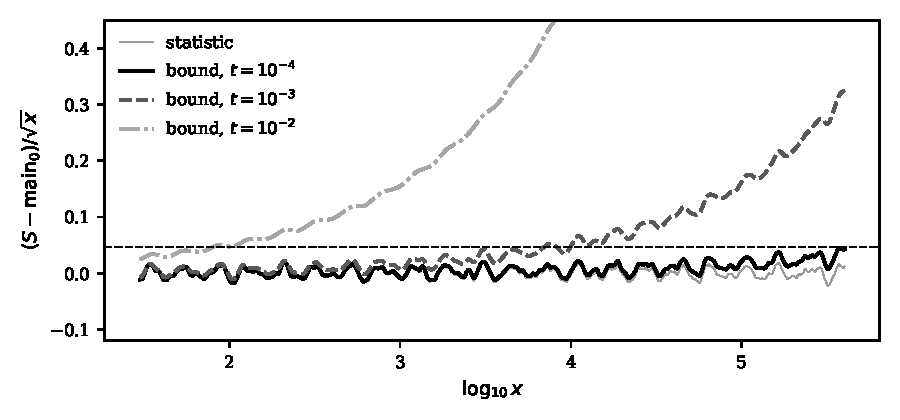
\includegraphics[width=\textwidth]{fig/gbm_bound.pdf}
\caption{The Riesz statistic of the primes less its main term, divided by $\sqrt x$, and the upper bounds of Corollary~\ref{gbm:cor:everyt} for three maturities, computed from the zeros. The dashed line is the sharp constant $c_0$. A long maturity gives a smooth bound that drifts upward.}\label{gbm:fig:bound}
\end{figure}

\section{The Chebyshev bound from zeros on the line up to a height}\label{gbm:sec:cheb}

\begin{theorem}[One sided bound from a partial Riemann hypothesis]\label{gbm:thm:cheb}
Suppose every nontrivial zero of $\zeta$ with $|\gamma|\le T_0$ is on the critical line. Suppose $T_0\ge8$. Then for every $x\ge2$ and every $\eta$ with $x^{-1}\le\eta\le1$,
\[
S(x)\le\mathrm{main}_0(x)+\bigl(c_0+0.047\,\eta\bigr)\sqrt x+\frac{x\,(\log x+2\log(1/\eta))}{2T_0^2}+\varepsilon ,
\]
with $\varepsilon=4\exp(-T_0^2\log x/24)$.
\end{theorem}

\begin{proof}
In Corollary~\ref{gbm:cor:everyt} split the zeros. Those on the line contribute at most $\sqrt x\sum w_\gamma e^{-t/8}\le\sqrt x\sum_{\rm on}a_\rho$ in absolute value. A zero off the line has $|\gamma|>T_0$ and $\mathrm{Re}\,\rho(1-\rho)=\beta(1-\beta)+\gamma^2\ge\gamma^2$, so its term is at most $|a_\rho|\,x\,e^{-tT_0^2/2}$. Now $c_0=\sum_{\rm on}a_\rho+\sum_{\rm off}\mathrm{Re}\,a_\rho$ and $|a_\rho|\le\sqrt{1+\gamma^{-2}}\,\mathrm{Re}\,a_\rho\le1.01\,\mathrm{Re}\,a_\rho$ for $|\gamma|\ge8$, so $\sum_{\rm off}|a_\rho|\le1.01c_0<0.047$ and the whole sum is at most $c_0\sqrt x+0.047\,x\,e^{-tT_0^2/2}$. Take $t=(\log x+2\log(1/\eta))/T_0^2$, so that $x\,e^{-tT_0^2/2}=\eta\sqrt x$; then $t\le3\log x/T_0^2\le\log x$, and the last term of the corollary is at most $4\exp(-T_0^2\log x/24)$.
\end{proof}

By the theorem of Platt and Trudgian \cite{PT21}, the hypothesis holds with $T_0=3\cdot10^{12}$. Then $1/(2T_0^2)=5.56\cdot10^{-26}$ and $\varepsilon$ is negligible.

\begin{corollary}[The square root bound for the Riesz statistic of $\zeta$]\label{gbm:cor:zeta}
Without hypothesis, with $G(x)=S(x)-\mathrm{main}_0(x)$:
\begin{enumerate}
\item for all $x\ge2$, $G(x)\le0.094\sqrt x+5.6\cdot10^{-26}\,x\log x$;
\item $G(x)\le(c_0+0.01)\sqrt x<0.0562\sqrt x$ for $2\le x\le10^{42}$;
\item $G(x)\le(c_0+1)\sqrt x$ for $2\le x\le10^{46}$.
\end{enumerate}
\end{corollary}

\begin{proof}
Take $\eta=1$ for the first. For the others choose $\eta$ and solve $0.047\eta\sqrt x+x(\log x+2\log(1/\eta))/(2T_0^2)\le\delta\sqrt x$ with $\delta=0.01$ and $\delta=1$; the largest admissible $x$ are $10^{42.4}$ and $10^{46.4}$ (computed). Since $\eta\ge x^{-1}$, the second needs $x\ge5$. For $2\le x<5$ the bound follows from the explicit formula at $t=0$: with zeros on the line up to $T_0$, $G(x)\le c_0\sqrt x+x\sum_{|\gamma|>T_0}|a_\rho|$, and the tail is below $2.96\cdot10^{-12}$ (the tail bound used in Theorem~\ref{st:thm:cert}), so the excess is below $0.01\sqrt x$.
\end{proof}

The sharp one sided bound $G(x)\le c_0\sqrt x$ is equivalent to the Riemann hypothesis when asked for all $x$ (Theorem~\ref{qt:thm:sharp}); Corollary~\ref{gbm:cor:zeta} shows it within a small excess up to $10^{42}$. Theorem~\ref{st:thm:cert} is stronger on its range, $G(x)<c_0\sqrt x-\mathrm{tr}(x)$ for $1<x\le3.49\cdot10^{45}$, from 300 certified low zeros; the bound above uses no phase of any low zero and is explicit for every $x$.

The qualitative form of Theorem~\ref{gbm:thm:cheb} for the family of (M) is Theorem~\ref{mq:thm:finiteheight}, whose proof is the same Jensen upgrade (Lemma~\ref{st:lem:upgrade}) with positive smoothing by a kernel of compact Fourier support, and which, under the floor hypothesis of that chapter and for $x\ge256$, needs the zeros only to height $x^{1/4}$; Proposition~\ref{mq:prop:jensen} shows that $x^{1/4}$ is the natural height for a positive average. What is added here is the explicit kernel and the explicit constants. B\"uthe \cite{Buthe16} turns zeros on the line up to height $T$ into the two sided bound for the unsmoothed $\psi$ of Schoenfeld for $4.92\sqrt{x/\log x}\le T$, a range of order $T^2\log T$, approximately $10^{25}$ for $T=3\cdot10^{12}$. Ours is an integrated ramp on one side, so the ranges do not compare as like with like; the range here is $x\approx T^4/\log^2T$, because of the smoothing, which gives the weights $1/\gamma^2$, and convexity, which makes the cost of averaging second order (Figure~\ref{gbm:fig:ranges}). We have not compared the kernels of \cite{Buthe16,Buthe18} with ours, and a specialist should do so before any bound here is quoted as new.

\begin{figure}[ht]
\centering
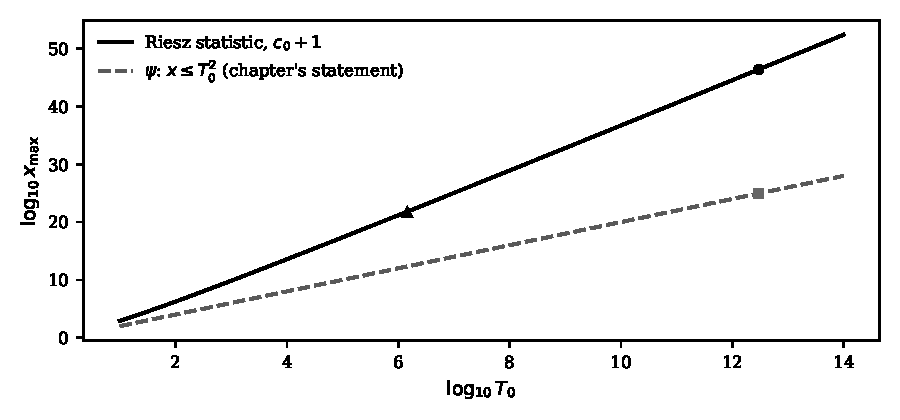
\includegraphics[width=\textwidth]{fig/gbm_ranges.pdf}
\caption{The range of $x$ on which a square root bound follows from zeros on the line up to height $T_0$: the one sided bound with constant $c_0+1$ for the Riesz statistic, by Theorem~\ref{gbm:thm:cheb}, and the two sided bound for $\psi$ by the criterion of B\"uthe. The points are $\zeta$ with $T_0=3\cdot10^{12}$ and the family $(3,23)$ with $T_0=10^8/69$.}\label{gbm:fig:ranges}
\end{figure}

\section{The family of (M)}\label{gbm:sec:family}

For the weight $w_+=(1+\chi_q)(1-\chi_d)$ the statistic is convex because $w_+\ge0$. Let $C=\sum_\chi c_\chi$, the sum of the four unsigned masses, and $\mathrm{main}_+(x)=x\log x-A_+x-\log x+K_+$ in the normalisation of Part E of the chapter on (M) (Section~\ref{mqf:sec:parte}), which differs from that of Theorem~\ref{mq:thm:fullweight} by elementary terms.

\begin{theorem}[The family]\label{gbm:thm:family}
Let $(q,d)$ be an admissible pair and suppose every nontrivial zero of the four functions $\zeta$, $L(\chi_q)$, $L(\chi_d)$, $L(\chi_q\chi_d)$ with $|\gamma|\le T_0$ is on the critical line, real zeros included. Suppose $T_0\ge8$. Then for every $x\ge2$ and $x^{-1}\le\eta\le1$,
\[
\begin{aligned}
S_{w_+}(x)\le{}&\mathrm{main}_+(x)+C\,(1+1.01\,\eta)\sqrt x\\&+\frac{(x+1)(\log x+2\log(1/\eta))}{2T_0^2}+\varepsilon ,
\end{aligned}
\]
with $\varepsilon\le(|A_+|+|K_+|+2C+2+\log x)\exp(-T_0^2\log x/48)$.
\end{theorem}

\begin{proof}
As before. The explicit formula is $S_{w_+}=\mathrm{main}_+ +\sum_P\sum_\rho a_\rho x^\rho-\sum_N\sum_\rho a_\rho x^\rho$ for $x\ge1$, the terms of the trivial zeros cancelling in pairs for this sign ($\zeta$ against $\chi_q\chi_d$, which are both even, and $\chi_q$ against $\chi_d$, both odd). The average of $-\log X_t$ is $-\log x+\frac12t$, which adds $\frac12t$ to the entropy. The zeros on the line contribute at most $\sqrt x$ times the sum of their weights in either group, and those off the line at most $1.01\,C\,x\,e^{-tT_0^2/2}$. On $X_t<1$ the function $\mathrm{main}_++\sum_P\sum_\rho a_\rho y^\rho-\sum_N\sum_\rho a_\rho y^\rho$ is bounded by $|A_+|+|K_+|+2C+1+|\log X_t|$, and $\mathbb E[|\log X_t|;X_t<1]\le(1+\log x)\,\mathbb P(X_t<1)^{1/2}$ by the inequality of Cauchy and Schwarz.
\end{proof}

For conductors up to $400000$ Platt \cite{Platt16} has verified the hypothesis to height $10^8/k$ for the conductor $k$. For $(3,23)$ the smallest of the four heights is that of the conductor $69$, $T_0=10^8/69\simeq1.449\cdot10^6$, and $C=1.9676$.

\begin{corollary}[(M) for the pair $(3,23)$ on a range]\label{gbm:cor:family}
Without hypothesis, for the weight $(1+\chi_3)(1-\chi_{23})$:
\begin{enumerate}
\item for all $x\ge2$, $S_{w_+}(x)\le\mathrm{main}_+(x)+3.96\sqrt x+2.4\cdot10^{-13}\,(x+1)\log x$;
\item $S_{w_+}(x)\le\mathrm{main}_+(x)+(C+0.01)\sqrt x$ for $200\le x\le4\cdot10^{17}$;
\item $S_{w_+}(x)\le\mathrm{main}_+(x)+(C+1)\sqrt x$ for $2\le x\le4\cdot10^{21}$.
\end{enumerate}
\end{corollary}

The limits of the second and third items are computed as $4.9\cdot10^{17}$ and $4.9\cdot10^{21}$, and the printed ones are rounded down. In the second item, $1.01C\eta\le0.01$ forces $\eta\le0.005$ and so $x\ge200$ by the condition $\eta\ge x^{-1}$; for $2\le x<200$ the bound follows from the slack computed from the primes on $1\le x\le4\cdot10^9$ (Section~\ref{mqf:sec:slack}, a floating point computation and not a theorem), which is positive there. That computation gives a positive slack on its range; the present bound gives no positive slack, but reaches about eight and twelve orders of magnitude further.

\section{The Thorin form: Gamma probes}\label{gbm:sec:gamma}

In the Thorin form of Problem (M) one asks that $F(b)=\int_0^\infty e^{-bu}\Phi(u)\,du$ be completely monotone on $b>\frac12$, where $\Phi(u)=c_0-\sum_\rho a_\rho e^{(\rho-\frac12)u}$ is the slack. The inequality of order $k$ at $b$ says that the mean of the slack under the Gamma law of shape $k+1$ and rate $b$ is nonnegative; the identity is Section~\ref{mqt:sub:reciprocal}. The Gamma variable is a sum of $k+1$ exponentials, so $e^U$ is a product of $k+1$ independent Pareto variables.

The book already proves these inequalities on a larger range than the quartet argument of the source draft gives. By Theorem~\ref{st:thm:disc} the inequalities of every order $k$ hold at rate $s$ as soon as the disc $|\rho-(\frac12+s)|<s$ is free of zeros. If every zero with $|\gamma|\le T_0$ is on the line, every zero off the line is outside that disc for $s\le T_0^2+\frac14$, so with $T_0=3\cdot10^{12}$ every inequality of Problem (M) in Thorin form for $\zeta$ with rate up to $T_0^2=9\cdot10^{24}$ is a theorem, for all orders $k$ (Corollary~\ref{st:cor:principle}). The quartet argument gives the range $b\le\frac12T_0^2$ and applies to the signed family as well (about $10^{12}$ for the family with $T_0=10^8/69$): a pair $\frac12\pm i\gamma$ contributes $w_\gamma(1-\cos((k+1)\theta)\cos^{k+1}\theta)>0$ with $\tan\theta=\gamma/b$, and the four zeros $\frac12\pm\delta\pm i\gamma$ of an off line zero have moduli at most $1-\frac12\gamma^{-2}$ for $b\le\frac12\gamma^2$, so their sum is nonnegative. So the content of Problem (M) lies at rates above $T_0^2$, and complete monotonicity on a bounded interval does not extend beyond it: the function $(L-b)^n$, $n\ge1$, is completely monotone on $b<L$ and not beyond.

Jensen's inequality with the Gamma law in place of the lognormal one gives a Chebyshev bound with no boundary term; it is Theorem~\ref{gbm:thm:gammakernel} below.

\section{The stopped martingale strategy in general}\label{gbm:sec:strategy}

Let $\tau$ be a stopping time of the motion for which $X_{t\wedge\tau}$ is uniformly integrable. The submartingale inequality gives $S_w(x)\le\mathbb E\,S_w(X_\tau)$, and three identities describe the right side.

\begin{theorem}[The strategy]\label{gbm:thm:strategy}
Let $\mu$ be the law of $X_\tau$, with mean $x$ and support in $[1,\infty)$, and let $\tilde\mu(dy)=(y/x)\mu(dy)$ be its size biased law. Then for $\zeta$
\[
S(x)\le\mathrm{main}_0(x)+\mathcal E(\mu)+\sum_\rho a_\rho\,\mathbb E\,X_\tau^\rho ,
\]
where the cost is
\[
\mathcal E(\mu)=\mathbb E[X_\tau\log X_\tau]-x\log x=\tfrac12\,\mathbb E\int_0^\tau X_s\,ds=x\,\mathrm{KL}(\tilde\mu\,\|\,\mu),
\]
and for every zero $\mathbb E\bigl[X_\tau^\rho\,e^{\tau\rho(1-\rho)/2}\bigr]=x^\rho$ when $\tau$ is bounded. Conversely every law on $(0,\infty)$ with mean $x$ and finite cost is the law of $X_\tau$ for some stopping time with $X_{t\wedge\tau}$ uniformly integrable.
\end{theorem}

\begin{proof}
The inequality is Jensen's with the explicit formula. By the formula of It\^o, $d(X\log X)=(1+\log X)\,dX+\frac12X\,dt$, which gives the second expression for the cost: stop first at $t\wedge\tau$ and localise; conditional Jensen for the bounded below function $y\log y$ and the integrability of $X_\tau\log X_\tau$ give uniform integrability of the entropy terms, and monotone convergence applies to the clock integral. The third expression is the definition of the divergence, since $d\tilde\mu/d\mu=y/x$. The identity for a zero is optional stopping for the exponential martingale of Wald. The converse is the embedding theorem of Skorokhod for the martingale $X$ in natural scale.
\end{proof}

So the strategy has exactly one freedom, the law $\mu$; the cost does not depend on which stopping time realises it. Under the size biased law write $V=\log(X_\tau/x)$; then $\mathbb E_{\tilde\mu}e^{-V}=1$, the cost is $x\,\mathbb E_{\tilde\mu}[V+e^{-V}-1]$, about $\frac12x\,\mathrm{Var}(V)$ for a narrow law, and the factor of a zero at $1+i\gamma$ is $x^{1+i\gamma}$ times the characteristic function of $V$ at $\gamma$, equal to $x$ times it in modulus.

\subsection{Three stopping rules}

\emph{A fixed time.} This is the lognormal law of Theorem~\ref{gbm:thm:cheb}.

\emph{Hitting times of levels.} If $\tau$ is the exit time of an interval $[xe^{-h},xe^{h}]$, then $X_\tau$ takes two values and the inequality is the chord inequality for a convex function. Its Mellin transform is almost periodic in $\gamma$ and returns arbitrarily near its largest value; the same holds for any rule whose law is carried by finitely many points. So pure hitting times of levels damp nothing: damping needs the stopped value to be spread, not the clock.

\emph{Steps of Pareto type.} Let $U$ have the Gamma law of shape $m$ and rate $\beta>1$. Then $X=e^U$ is a product of $m$ independent Pareto variables, with mean $x=(\beta/(\beta-1))^m$, and $X\ge1$. The price of the prime portfolio under this law is exact, with the regularised upper incomplete Gamma function $Q$ in the place of the normal distribution function:
\begin{equation}\label{gbm:eq:gammaprice}
\begin{aligned}
&\sum_n\frac{\Lambda(n)}n\Bigl(x\,Q(m,(\beta-1)\log n)-n\,Q(m,\beta\log n)\Bigr)\\
&\qquad=\frac{xm}{\beta-1}-(1+\gamma_E)x+\log2\pi-\sum_{j\ge1}\frac{(1+2j/\beta)^{-m}}{2j(2j+1)}\\
&\qquad\quad+\sum_\rho a_\rho\Bigl(1-\frac\rho\beta\Bigr)^{-m}.
\end{aligned}
\end{equation}
There is no boundary term. The proof is that of Theorem~\ref{gbm:thm:price}: tilting the Gamma law of rate $\beta$ to rate $\beta-1$ gives $\mathbb E[X;X>n]=x\,Q(m,(\beta-1)\log n)$, and $\mathbb E[X\log X]=xm/(\beta-1)$, $\mathbb E\,X^{-2j}=(1+2j/\beta)^{-m}$, $\mathbb E\,X^\rho=(1-\rho/\beta)^{-m}$, with the explicit formula valid on the whole support since $X\ge1$. Both sides of~\eqref{gbm:eq:gammaprice} were computed on the primes (for $m=1000$, $\beta=125$: $19972.4731$, against $S(x)=19873.9062$ at $x=3078.42$).

\begin{theorem}[The bound from the Gamma kernel]\label{gbm:thm:gammakernel}
Suppose every nontrivial zero of $\zeta$ with $|\gamma|\le T_0$ is on the line, with $T_0\ge30$. For $x\ge2$ and $x^{-1}\le\eta\le1$,
\[
S(x)\le\mathrm{main}_0(x)+\bigl(c_0+0.047\,\eta\bigr)\sqrt x+\frac{x\,(\log x+2\log(1/\eta))}{2T_0^2-66},
\]
with no further term.
\end{theorem}

\begin{proof}
Put $\lambda=1+2\log(1/\eta)/\log x\le3$ and $\beta_m=(1-x^{-1/m})^{-1}$, the rate for which the mean is $x$. The $\beta_m$ increase from $\beta_1\le2$ in steps of at most $1/\log x$, so there is an $m$ with $T_0^2/\lambda-3\lambda-1.45\le\beta_m-1\le T_0^2/\lambda-3\lambda$; take $\beta=\beta_m$. For a zero off the line, $(1-\sigma/\beta)^2+\gamma^2/\beta^2\ge((\beta-1)^2+T_0^2)/\beta^2$, so $|\mathbb E\,X^\rho|\le x\,(1+T_0^2/(\beta-1)^2)^{-m/2}$. Since $m\ge(\beta-1)\log x$ and $\log(1+y)\ge y(1-\frac12y)$, the choice of $\beta$ makes this at most $\eta\sqrt x$. The zeros on the line contribute at most $\sqrt x\sum_{\rm on}a_\rho$, since $|\mathbb E X^\rho|\le\sqrt x$ there. The cost is $xm(1/(\beta-1)-\log(\beta/(\beta-1)))\le x\log x/(2(\beta-1)-1)$.
\end{proof}

The Gamma kernel is as good as the lognormal one, with the same constant $\frac12$.

\subsection{Random clocks, and the Wald and van Dantzig view}

Let the maturity be a random time $\tau$ independent of the motion, with Laplace transform $\varphi_\tau$. Then $\mathbb E\,X_\tau^\rho=x^\rho\varphi_\tau(\rho(1-\rho)/2)$: the factor of a zero is the Laplace transform of the clock at the point $\frac18+\frac12\gamma^2$ of the Thorin measure, and the cost is $\frac12x\,\mathbb E\tau$. The stopped value and the clock satisfy the identity of Wald, $\mathbb E\exp(sB_\tau-s^2\tau/2)=1$, but are not a Wald couple in the sense of Definition~\ref{mw:def:wald}, since $B_\tau$ is not independent of $\tau$.

\begin{proposition}[Independent clocks do not help]\label{gbm:prop:clock}
For an independent clock and real $s\ge0$, $\varphi_\tau(s)\ge e^{-s\,\mathbb E\tau}$. So among independent clocks of given mean, hence of given cost, the constant one damps every zero on the critical line most.
\end{proposition}

\begin{proof}
Jensen's inequality for the convex function $e^{-s\tau}$, applied at $s=\frac18+\frac12\gamma^2$.
\end{proof}

The restriction to real $s$ is needed: for a zero off the line $s$ is complex, and a clock with two values can be chosen with $\varphi_\tau(s)=0$ at a given $s$. A Gamma clock, with $\varphi_\tau(s)=(1+s/\theta)^{-m}$, damps only like a power of the height. So the couples of Wald and the pairs of van Dantzig give no better kernels as independent clocks. They identify what the damping is: for the constant clock the factor $e^{-t(\frac18+\frac12\gamma^2)}$ is the survival probability at the maturity of the exponential variable attached to the zero $\gamma$ in the hitting time $\sum_\gamma e_\gamma/(\frac18+\frac12\gamma^2)$ (Theorem~\ref{mqt:thm:esscher}), and under RH the normalised zero sum in the price is $e^{-t/8}\,\mathbb E\,H(u+B_t)$, the function $H=c_0-\Phi$ smoothed by the Brownian motion itself. What does help is a clock that depends on the path.

\subsection{Kernels that are generalised gamma convolutions}

Let $U=\log X$ be a generalised gamma convolution in the sense of Thorin \cite{Thorin78}, with Thorin measure $\nu$ on $(1,\infty)$, a limit of sums of independent Gamma variables with rates $y$. With $z=1/(y-1)$,
\[
\log x=\int\log(1+z)\,\nu(dy),\qquad\frac{\mathcal E}x=\int\bigl(z-\log(1+z)\bigr)\nu(dy),
\]
\[
\frac{|\mathbb E\,X^{1+i\gamma}|}x=\exp\Bigl(-\tfrac12\int\log\bigl(1+\gamma^2z^2\bigr)\nu(dy)\Bigr).
\]
So each atom of the Thorin measure of the kernel has a cost $z-\log(1+z)$ and a damping $\frac12\log(1+T^2z^2)$ at height $T$.

\begin{proposition}[Optimality within the class]\label{gbm:prop:ggc}
For $T\ge2$ and all $z>0$, $z-\log(1+z)\ge(1-\frac2{9T^2})\,\log(1+T^2z^2)/(2T^2)$. Hence a kernel of this class with $|\mathbb E\,X^{1+iT_0}|\le\eta\sqrt x$ has cost at least $(1-\frac2{9T_0^2})\,x(\log x+2\log(1/\eta))/(2T_0^2)$, and Theorem~\ref{gbm:thm:gammakernel} is optimal in the class up to the factor $1+O(T_0^{-2})$.
\end{proposition}

\begin{proof}
Put $q=T^2$, $c=1-2/(9q)$ and $H(z)=z-\log(1+z)-\frac{c}{2q}\log(1+qz^2)$. Then $H'(z)=w(z)\,z\,(1-c-cz+qz^2)$ with $w(z)=[(1+z)(1+qz^2)]^{-1}$ decreasing. The primitive of $z(1-c-cz+qz^2)$ vanishing at $0$ is $J(z)=z^2[(1-c)/2-cz/3+qz^2/4]$, and the bracket is nonnegative because its discriminant is $c^2/9-(1-c)q/2=\frac19(c^2-1)\le0$. Integration by parts gives $H(z)=w(z)J(z)-\int_0^zw'(v)J(v)\,dv\ge0$. The consequence for the kernel follows by integrating against $\nu$ and using the three displayed formulas.
\end{proof}

The least ratio of the two sides, computed in high precision, is $0.9503$ at $T=2$ and $1-2.2222\cdot10^{-7}$ at $T=10^3$, which is $1-2/(9T^2)$ up to the digits shown; the inequality is sharp to leading order, with a double root at $z=2/(3T^2)$. The ratio of cost to damping is close to its least value for every rate $y$ much larger than $T$ and grows quickly below (Figure~\ref{gbm:fig:frontier}, left). So within the class all fine Gamma factors are equally efficient, the lognormal law is their limit after centring, and the logarithm in the cost cannot be removed within the class.
\subsection{A rule that removes the logarithm}

Outside the class one can expect to do better. The logarithm arises because a Gaussian characteristic function reaches the level $x^{-1/2}$ only at $\sqrt{\log x}$ standard deviations. A characteristic function that vanishes beyond $T$ has no such loss. What follows is an outline and is labelled so; it is not used elsewhere in the chapter.

\begin{remark}[Band limited kernel; outline, not a theorem]\label{gbm:rem:band}
Let $T=T_0-s$ and let $V$ have, under the size biased law, the density proportional to
\[
\Bigl(\frac{\cos(vT/2)}{\pi^2-v^2T^2}\Bigr)^2e^{-2\sqrt{1+v^2}},
\]
shifted so that $\mathbb E\,e^{-V}=1$. The first factor has a characteristic function supported in $[-T,T]$ and variance $\pi^2/T^2$, the least possible for that support; the second gives the exponential moments that the first lacks. The expected cost is $(\frac12\pi^2+o(1))\,x/T^2$, and $|\mathbb E\,X^{\sigma+i\gamma}|\le Ce^{-c(|\gamma|-T)}x^\sigma$ for $|\gamma|\ge T$ and $\frac12\le\sigma\le1$. Consequently, with $s$ a multiple of $\log x$, the hypothesis of Theorem~\ref{gbm:thm:cheb} would give
\[
S(x)\le\mathrm{main}_0(x)+(c_0+o(1))\sqrt x+\frac{5x}{T_0^2}
\]
for $\log x$ small compared with $T_0$.
\end{remark}

We computed this kernel for $T=20,60,200$: the cost times $T^2$ is $4.42$, $4.77$, $4.88$, tending to $\frac12\pi^2=4.93$, and at $T=200$ the Mellin transform falls from $3\cdot10^{-3}$ at $0.9T$ to $10^{-11}$ at $T+10$ (Figure~\ref{gbm:fig:frontier}, right). We have not written the estimates with explicit constants, so the displayed bound is not a theorem here. If it is confirmed it replaces $x\log x/(2T_0^2)$ by $5x/T_0^2$ and moves the ranges of Corollary~\ref{gbm:cor:zeta} from $10^{42}$ and $10^{46}$ to about $3\cdot10^{44}$ and $3\cdot10^{48}$ (computed from the displayed bound). The untapered cosine law with a rigorous truncation is in Lemma~\ref{st:lem:cosine}, with cost $4.9348/H^2$ at a fixed height $H$; we have not carried the displayed bound through it.

\begin{figure}[ht]
\centering
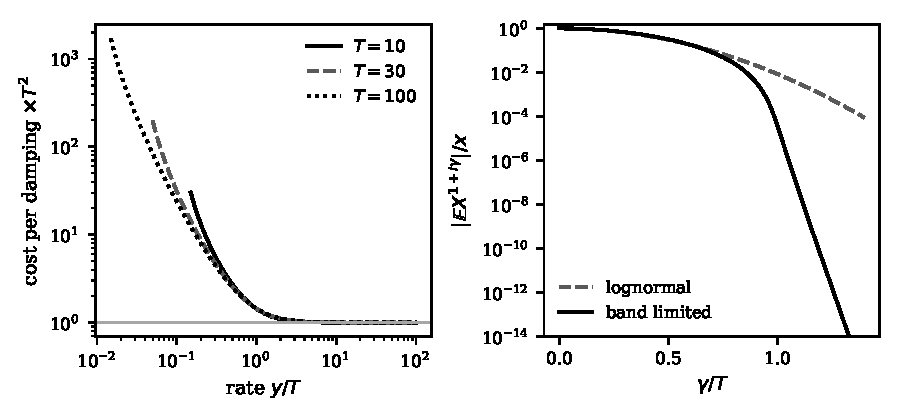
\includegraphics[width=\textwidth]{fig/gbm_gamma_frontier.pdf}
\caption{Left: the cost of a Gamma factor of rate $y$ per unit of damping at height $T$, times $T^2$; every rate well above $T$ is efficient and none goes below the limiting value $1-2/(9T^2)$. Right: the modulus of the Mellin transform on the line $\mathrm{Re}\,s=1$ for the lognormal kernel and for the band limited kernel of the same cost.}\label{gbm:fig:frontier}
\end{figure}

\subsection{The limit of the strategy}

\begin{theorem}[Lower bound for every stopping rule]\label{gbm:thm:lower}
Let $T\ge\frac12$ and let $\mu$ be any law on $(0,\infty)$ with mean $x$ such that $|\mathbb E\,X^{1+i\gamma}|\le\frac12x$ for all $|\gamma|\ge T$. Then $\mathcal E(\mu)\ge x/(192\,T^2)$.
\end{theorem}

\begin{proof}
Let $V,V'$ be independent with the size biased law and $D=V-V'$, and let $\varphi$ be the characteristic function of $V$. Then $\mathbb E[1-\cos TD]=1-|\varphi(T)|^2\ge\frac34$, and $1-\cos TD\le\min(2,\frac12T^2D^2)$, so $\mathbb P(|D|\ge1/T)\ge\frac16$. The function $\psi(v)=v+e^{-v}-1$ satisfies $\psi(v)\ge\frac14\min(v^2,|v|)$, and one of $|V|$, $|V'|$ is at least $\frac12|D|$; for $T\ge\frac12$ one has $\min(D^2/4,|D|/2)\ge1/(4T^2)$ on $|D|\ge1/T$, so $2\,\mathbb E\psi(V)\ge\frac16\cdot\frac14\cdot\frac1{4T^2}$. The cost is $x\,\mathbb E\psi(V)$.
\end{proof}

Without the hypothesis $T\ge\frac12$ the statement is false: a size biased law spread over a width of order $1/T$ costs of order $x/T$. This is Proposition~\ref{mq:prop:jensen} with the constant $192$ in place of $256$; the proof uses damping at one frequency only.

So the cost of any rule that protects against a zero near $1+iT_0$ lies between $x/(192T_0^2)$ and the $x\log x/(2T_0^2)$ of Theorem~\ref{gbm:thm:gammakernel}, and is of order $x/T_0^2$ if the band limited kernel is confirmed. The strategy turns the Riemann hypothesis up to height $T$ into the square root bound up to $x$ of order $T^4/\log^2T$, and no such rule reaches beyond order $T^4$ while the damping is asked at the edge height and the entropy is charged in full. To go beyond one must use information about the zeros above the verified height; we expect, but do not prove, that the classical zero free region gives a bound of the quality of the prime number theorem.

\subsection{Modulated Gamma probes}

A real Gamma probe sees a zero off the line only at rates above $\gamma^2/(2\delta)$ for a zero $\frac12+\delta+i\gamma$ (the pole at $\delta+i\gamma$ must be nearer to $b$ than the pole at the origin). A probe multiplied by a frequency sees it at any rate. Let $\psi_{m,b}(\tau)=\mathbb E[\Phi(U)e^{i\tau U}]$ with $U$ of shape $m$ and rate $b>\frac12$; then
\[
\psi_{m,b}(\tau)=c_0\Bigl(1-\frac{i\tau}b\Bigr)^{-m}-\sum_\rho a_\rho\Bigl(1-\frac{\rho-\frac12+i\tau}b\Bigr)^{-m}.
\]
If $\Phi\ge0$ then $\Phi$ times the Gamma density is a positive measure, $\psi_{m,b}$ is positive definite, and $|\psi_{m,b}(\tau)|\le\psi_{m,b}(0)$ for all $\tau$. The converse needs every order and every frequency at one rate.

\begin{proposition}[One rate suffices]\label{gbm:prop:modulated}
Fix $b>\frac12$. If $|\psi_{m,b}(\tau)|\le\psi_{m,b}(0)$ for every integer $m\ge1$ and every real $\tau$, then $\zeta$ has no zero with real part in $(\frac12,\frac12+2b)$, in particular none to the right of the critical line.
\end{proposition}

\begin{proof}
With $F$ as in Section~\ref{gbm:sec:gamma}, $\sum_{m\ge1}\psi_{m,b}(\tau)z^{m-1}=b\,F(b(1-z)-i\tau)$ near $z=0$. The partial fraction form of $F$ continues it meromorphically, with a pole of nonzero residue at each shifted zero. At $\tau=0$ the coefficients are nonnegative, and the function is regular on the segment $0\le z<1$ (a real zero of $\zeta$ in the strip does not exist), so by the theorem of Pringsheim, as in Theorem~\ref{st:thm:disc}(a), its radius of convergence is at least $1$. The hypothesis dominates the coefficients at every $\tau$ by those at $\tau=0$, so the radius is at least $1$ at every $\tau$. A zero $\frac12+h+i\gamma$ with $h>0$ would give, at $\tau=-\gamma$, an uncancelled pole at $z=1-h/b$ inside the unit disc when $0<h<2b$, a contradiction; since $b>\frac12$ this covers $(0,\frac12]$.
\end{proof}

The window criterion of the book, Corollary~\ref{mq:hyp:window} of Theorem~\ref{mq:thm:window}, is proved independently of any draft. Under the Riemann hypothesis $|\psi_{m,b}|$ has, as $m\to\infty$, a peak of height $a_\gamma/c_0$ at each zero, $a_\gamma=1/(\frac14+\gamma^2)$. From the primes below $4\cdot10^6$, with $m=24$ and $b=3$, the peaks of $|\psi(\tau)|/\psi(0)$ stand at the first four zeros $14.135,\ 21.02,\ 25.01,\ 30.425$ with heights $0.1082,\ 0.0490,\ 0.0346,\ 0.0234$, the predicted $a_\gamma/c_0$ (Figure~\ref{gbm:fig:spectro}). The maximum after $\tau=1$ is $0.28<1$.

\begin{figure}[ht]
\centering
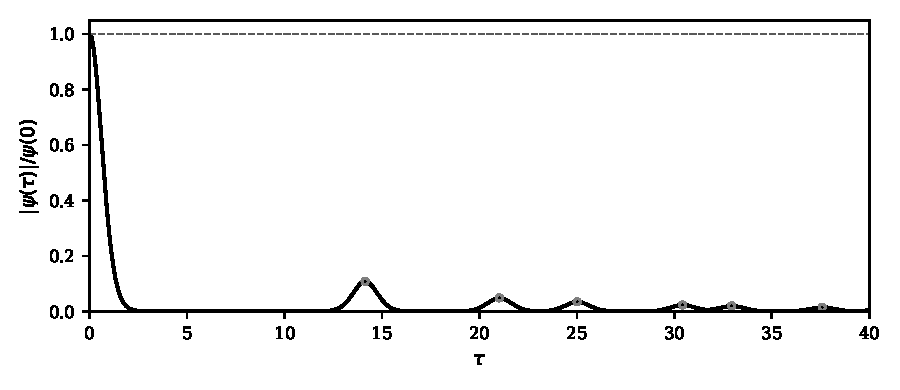
\includegraphics[width=\textwidth]{fig/gbm_gamma_spectroscopy.pdf}
\caption{The modulus of the modulated Gamma probe of the slack, shape $24$ and rate $3$, computed from the primes below $4\cdot10^6$ and divided by its value at frequency $0$. The peaks stand at the zeros of $\zeta$ with heights $a_\gamma/c_0$; the inequality $|\psi(\tau)|\le\psi(0)$ is the dashed line.}\label{gbm:fig:spectro}
\end{figure}

\section{Pricing the prime portfolio without zeros}\label{gbm:sec:nozeros}

Here the price of Theorem~\ref{gbm:thm:price} is obtained on the side of the integers, where no zero appears. There are three ways to do it, and their comparison is the intuition for (M).

\subsection{The integer portfolio}

Let $\Pi(x,t)=\sum_{n\ge1}\frac{\log n}n\,C(x,n,t)$, the price of the portfolio that holds $\log n/n$ calls at every integer $n$. Its intrinsic value is an average of logarithms of factorials, and that of the prime portfolio an average of logarithms of least common multiples:
\[
\begin{aligned}
\Pi(x,0)&=x\int_1^x\frac{\log(\lfloor y\rfloor!)}{y^2}\,dy,\\
S(x)&=x\int_1^x\frac{\log\mathrm{lcm}(1,\dots,\lfloor y\rfloor)}{y^2}\,dy .
\end{aligned}
\]
Both follow from $(x/n-1)_+=x\int_n^xy^{-2}dy$ for $n\le x$, the identity $\sum_{n\le y}\log n=\log\lfloor y\rfloor!$ and $\psi=\log\mathrm{lcm}$.
\begin{theorem}[Price of the integer portfolio]\label{gbm:thm:integer}
Let $a=\log x+\frac12t$ and let $\gamma_1=-0.0728158$ be the first Stieltjes constant. For $x\ge1$ and $0<t\le1$,
\[
\Pi(x,t)=x\Bigl(\tfrac12a^2-a+1+\tfrac12t+\gamma_1\Bigr)-\tfrac12\log2\pi+\varepsilon(x,t),
\]
where $\varepsilon(x,t)=O_N(x^{-N}t^{-N})$ for every $N\ge1$.
\end{theorem}

\begin{proof}
Since $\mathbb E\,X_t^s=x^se^{ts(s-1)/2}$ and $(y-1)_+=\frac1{2\pi i}\int y^s\,ds/(s(s-1))$ on a line to the right of $1$,
\[
\Pi(x,t)=\frac1{2\pi i}\int\frac{-\zeta'(s)\,x^s\,e^{ts(s-1)/2}}{s(s-1)}\,ds .
\]
The integrand has a triple pole at $s=1$, where $-\zeta'(s)=(s-1)^{-2}+\gamma_1+\cdots$, with residue $x(\frac12a^2-a+1+\frac12t+\gamma_1)$, and a simple pole at $s=0$ with residue $\zeta'(0)=-\frac12\log2\pi$. It has no other pole, because $\zeta'$ is regular elsewhere: the zeros of $\zeta$ play no part. On the line $\mathrm{Re}\,s=-N$ the integrand is $O_N(x^{-N}(1+|\tau|)^{N-3/2}\log(2+|\tau|)\,e^{-t\tau^2/2})$.
\end{proof}

The remainder $\varepsilon$ must be kept whenever the expansion is inserted in a sum. The two sides agree to below $10^{-9}$ (for $x=1000$ and $t=10^{-2}$ both are $17911.602711$, recomputed).

\subsection{The hedge of M\"obius}

\begin{theorem}[Chebyshev's identity for prices]\label{gbm:thm:moebius}
For all $x>0$ and $t>0$,
\[
\sum_{m\ge1}P(x/m,t)=\Pi(x,t),\qquad P(x,t)=\sum_{m\ge1}\mu(m)\,\Pi(x/m,t),
\]
both series converging absolutely. More generally, if $e$ is a function of finite support on the positive integers and $c_m=\sum_{d\mid m}e_d$, then $\sum_de_d\,\Pi(x/d,t)=\sum_mc_m\,P(x/m,t)$.
\end{theorem}

\begin{proof}
The price of a call is homogeneous: $C(x,nm,t)=m\,C(x/m,n,t)$. So $\frac{\Lambda(n)}n\,C(x/m,n,t)=\frac{\Lambda(n)}{nm}\,C(x,nm,t)$, and summing over $nm=k$ with $\sum_{n\mid k}\Lambda(n)=\log k$ gives the first identity; the second is the inversion of M\"obius and the third is the same computation with $e$. For convergence, $C(y,n,t)\le y\exp(-(\log(n/y)-\frac12t)^2/(2t))$ when $n>ye^{t/2}$, so the terms with $m>xe^{t}$ decrease faster than any power.
\end{proof}

This is the price form of the identity of Chebyshev for the integer portfolio (Theorem~\ref{ct:thm:mobius}). The prime portfolio is hedged exactly by integer portfolios started at the levels $x/m$, long or short according to $\mu(m)$, and each of these has an elementary price. For $x=1000$ and $t=10^{-2}$ the sum of $2227$ terms is $5337.271787$, the price found from the primes and from the zeros (recomputed). No zero appears, but the hedge is signed, and the whole difficulty has moved into the cancellation. Inserting Theorem~\ref{gbm:thm:integer} for the terms with $m\le M$, the terms proportional to $x/m$ give $x\log x-(1+\gamma_E)x+\frac12xt$ from the three series $\sum\mu(m)/m=0$, $\sum\mu(m)\log m/m=-1$, $\sum\mu(m)\log^2m/m=-2\gamma_E$; the constant $\log2\pi$ of the main term does not come from these series (the sum $\sum\mu(m)$ does not converge as an ordinary series), and it requires the truncation, the contour remainders and the tail $m>M$ to be kept together.

\subsection{Chebyshev's inequalities for the price}

A hedge with few terms and a sign pattern gives inequalities. This is the method of Chebyshev; for prices it has no rounding errors, because Theorem~\ref{gbm:thm:integer} is exact up to the remainder $\varepsilon$.

\begin{theorem}[Chebyshev's inequalities for the price]\label{gbm:thm:chebprice}
Let $e$ have finite support with $\sum e_d/d=0$, put $A_e=-\sum e_d\log d/d$, $B_e=\sum e_d\log^2d/d$ and, for $x\ge\max\mathrm{supp}\,e$ and $0<t\le1$,
\[
\begin{aligned}
L_e(x,t)&=\sum_de_d\,\Pi(x/d,t)\\&=A_e\,x\,(a-1)+\tfrac12B_e\,x\\&\quad-\tfrac12\log2\pi\sum_de_d+\varepsilon_e .
\end{aligned}
\]
The price $P(\cdot,t)$ is nonnegative and increasing. Hence, with $e=(1,-2)$ on $\{1,2\}$,
\[
L_e(x,t)\le P(x,t)\le L_e(x,t)+P(x/2,t),\quad A_e=\log2,
\]
and with the choice of Chebyshev (Proposition~\ref{ct:prop:cheb1850}), $e=(1,-1,-1,-1,1)$ on $\{1,2,3,5,30\}$,
\[
L_e(x,t)\le P(x,t)\le L_e(x,t)+P(x/6,t),\qquad A_e=0.92129 .
\]
Iterating, $A_e\,x\log x\,(1+o(1))\le P(x,t)\le\frac65A_e\,x\log x\,(1+o(1))$ at fixed $t$, with $\frac65A_e=1.10555$.
\end{theorem}

\begin{proof}
In the first case $c_m=(-1)^{m+1}$, and an alternating series of decreasing terms lies between its first term and its first two. In the second, $c_m$ has period $30$, takes the values $1,0,-1$, and alternates in sign over its nonzero values beginning $c_1=1$, $c_6=-1$.
\end{proof}

The constants $0.92129$ and $1.10555$ are those of Proposition~\ref{ct:prop:cheb1850} and Theorem~\ref{ct:thm:chebggc}, transferred to the smoothed payoff; the price form is what is new here. For $x=10^5$ and $t=10^{-3}$ the price is $993624$ and the ratios of the lower and the iterated upper bound to it are $0.936$ and $1.083$, within the constants. A hedge with finitely many terms goes no further without the prime number theorem.

\subsection{The equation of Black and Scholes, and the Greeks}

\begin{theorem}[The Greeks of the prime portfolio]\label{gbm:thm:greeks}
The price satisfies $\partial_tP=\frac12x^2\partial_x^2P$ with $P(x,0)=S(x)$, where $t$ is the time to maturity. Its delta, gamma and theta are
\[
\partial_xP=\sum_n\frac{\Lambda(n)}n\,N(d_1(n)),\qquad x\,\partial_x^2P=\vartheta_t(x),\qquad\partial_tP=\tfrac12x\,\vartheta_t(x),
\]
where $\vartheta_t(x)=\sum_n\frac{\Lambda(n)}n\,\frac{N'(d_1(n))}{\sqrt t}$ is the density of the prime powers in the log strike, weighted by $\Lambda$, seen through a Gaussian window of width $\sqrt t$ centred at $\log x+\frac12t$. Consequently the time value is
\[
P(x,t)-S(x)=\frac x2\int_0^t\vartheta_s(x)\,ds .
\]
\end{theorem}

\begin{proof}
Each call satisfies the equation, and its gamma is $N'(d_1)/(x\sqrt t)$.
\end{proof}

The delta is a smoothed $\sum_{n\le x}\Lambda(n)/n$, close to $\log x-\gamma_E+\frac12t$; the gamma is a smoothed density of primes, close to $1/x$ by the prime number theorem; the theta is half of $x$ times that density. At $x=10^5$ and $t=10^{-3}$ the time value is $49.79$ against $\frac12xt=50$ (recomputed). The identity $S=P-\frac x2\int_0^t\vartheta_s\,ds\le P$ is exact. A sieve bound for $\vartheta$ from the theorem of Montgomery and Vaughan \cite{MV73}, $\pi(y+h)-\pi(y)\le2h/\log h$, would give a lower bound for $S$ in terms of $P$, but we do not claim one: it needs a stated range of $x$ and $t$, and without one it fails (for fixed $x$ and large $t$ the time value is of order $xt/2$).

\section{Three ways to price, and what (M) is}\label{gbm:sec:threeways}

\emph{The signed hedge.} Theorem~\ref{gbm:thm:moebius} prices the portfolio exactly with integer portfolios, long and short. Everything is elementary except the cancellation among the positions. A proof of the square root bound by this route is a proof of the bound $\sum_{n\le x}\mu(n)=O(x^{1/2+\varepsilon})$ for the function of M\"obius, which is the classical equivalent of RH.

\emph{Super replication.} If only long positions are allowed, the cheapest portfolio that dominates the primes is expected to be given by the sieve, and to cost about twice the price: this is the constant $2$ of Brun and Titchmarsh, and the factor two is Selberg's parity principle, a heuristic limit of sieve majorants, not a theorem about portfolios. In the language of the market there would be a spread of a factor two between the fair price and the cost of dominating the portfolio with positive holdings in arithmetic progressions. Chebyshev's hedge of Theorem~\ref{gbm:thm:chebprice} has a narrower spread, $0.92$ to $1.11$, because it is allowed a few short positions. We prove nothing about the cheapest positive superhedge.

\emph{The product formula.} The third way does not hedge. If $D$ is a nonzero integer then $\sum_pv_p(D)\log p=\log|D|$, so a sum over primes of valuations is at most the logarithm of a size. Chebyshev used the integer $\lfloor x\rfloor!\lfloor x/30\rfloor!/(\lfloor x/2\rfloor!\lfloor x/3\rfloor!\lfloor x/5\rfloor!)$ (Proposition~\ref{ct:prop:cheb1850}), which is exactly the hedge of Theorem~\ref{gbm:thm:chebprice} and so the product formula applied to a signed integer; the central binomial coefficient, whose valuations are $1$ at the primes between $n$ and $2n$, is the simplest integer of this kind, and gives an upper bound of the right order with no knowledge of cancellation. A ramp sum is of the same kind when an integer can be found whose valuation at $p$ is at least $\sum_h(a/p^h-w)_+$: the value of the portfolio is then at most the logarithm of the size of that integer. This is the structure of the claimed proof explained in \cite{Rub26}, Chebyshev's argument run with a far better integer, which must have exponents smooth in $p^h$ with no floor function, a size known through its linear term to a relative accuracy $x^{-1/2}$, and a set of primes that can be related to all primes. The integers are derivatives of theta functions of lattices with complex multiplication; their valuations at the inert primes are ramps; the weight $(1+\chi_q)(1-\chi_d)$ records which primes are inert and in which cell they fall; and the bound is one sided because divisibility bounds a valuation below and size bounds the total above. In this picture (M) says that the size of those integers is known to within a factor $\exp(x^{1/2+\varepsilon})$. This describes what \cite{Rub26} reports; it is not checked here.

So the intuition for (M) without zeros is this. The value of the prime portfolio is the logarithm of the part of an integer that the counted primes must divide. A hedge needs cancellation, domination with positive weights is expected to lose a factor two, but an integer cannot be more divisible than it is large, so a sharp size bounds the value from above with no cancellation. The weight of the claimed proof is on two statements: that the divisibility is as large as the ramps say, which is hypothesis (B) of \cite{Rub26}, and that the size is as small as the main term says, an estimate for theta functions. Neither is within the methods of this chapter, which adds that once any upper bound of this kind is available on windows, the stopped martingale strategy and the window criterion (Theorem~\ref{mq:thm:window}) turn it into information about zeros.

\subsection{A worked example of the third way: the lemniscate}

Version 2 of \cite{Rub26} gives a proof of the simplest instance, which we have not checked (the book's own form, with the valuation bound of Theorem~\ref{mql:thm:div} in place of Le18, is Remark~\ref{mql:rem:toy}), and it is worth setting it in the present language, because it shows the third way working and failing at once. Let $A_n$ be the $n$th derivative of the lemniscate sine at the origin, a nonzero integer for $n\equiv1\pmod4$. At every prime $p\equiv3\pmod4$, inert in $\mathbb Q(i)$, Theorem Le18 of \cite{Rub26} asserts $v_p(A_n)\ge\lfloor np/(p^2-1)\rfloor$, and $np/(p^2-1)=n(p^{-1}+p^{-3}+\cdots)$ is a sum over the odd powers of $p$ with no floor inside. The product formula then gives, for the floored valuations and with $v_2(A_n)=(n-1)/2$, and Theorem Le9 of \cite{Rub26} asserts the size:
\[
\begin{aligned}
&\sum_{p\equiv3\,(4)}\Bigl\lfloor\frac{np}{p^2-1}\Bigr\rfloor\log p+\frac{n-1}2\log2\\&\qquad\le\log n!-(n+1)\log\frac\varpi{\sqrt2}+\log4+o(1).\end{aligned}
\]
The right side is $n\log n+O(n)$ and the left side is $\frac12n\log n+O(n)$. By the authors' computation from the formulas of \cite{Rub26}, at $n=2001$ the inert primes account for $6188.3$ of $11979.5$ (the sums are of valuations as reported there). Granted Le18 and Le9, the bound is valid, needs no cancellation, and is too large by a factor two: it bounds the portfolio by the size of a whole integer, and this integer is twice as large as the part that the counted primes explain.

The three defects that \cite{Rub26} reads off are exactly what separates this example from (M): the floor loses about one unit at each prime, which is of the order of the linear term; only the inert primes are counted; and the size is that of a function with a pole at finite distance, $n!$, where a function of Gaussian growth would give $\sqrt{n!}$ and close the factor two. The claimed proof replaces the single integer by a map between lattices, the function by theta series, and one derivative by a chain of $m$ lifts.

\subsection{The exponent, and a weaker target}

The draft explains where the exponent one half comes from. After normalisation the errors in (M) are of two kinds: an error $x/m$ made once, at the two ends of a chain of $m$ lifts, and an error $m$ accumulated along the chain. They balance at $m\approx\sqrt x$. The draft adds that if the accumulated cost were $m^2$, the balance would be at $m=x^{1/3}$ with error $x^{2/3}$, giving no zero with real part above $\frac23$ if the inequality could be proved. By the window criterion with $\theta=\frac23$ (Section~\ref{mq:sec:onewindow}), it is enough that $G(x)\le x^{2/3+\varepsilon}$ on windows $[Y,Y^{3/2}]$ for every $\varepsilon>0$ and arbitrarily large $Y$, or the subpower prefactor of Theorem~\ref{mq:thm:window}; in terms of the slack, that $\Phi(u)\ge-e^{(\frac16+\varepsilon)u}$ on windows; and in terms of the portfolio, that its value exceed the elementary part of its price by at most $x^{2/3+\varepsilon}$. The stopped martingale strategy reaches such a bound for $x$ up to about $(2T_0^2/\log x)^3$, where the cost $x\log x/(2T_0^2)$ of Theorem~\ref{gbm:thm:gammakernel} is below $x^{2/3}$, which is about $10^{69}$ for $\zeta$ (about $6\cdot10^{72}$ with the cost $5x/T_0^2$ of the outline); this is a finite range again and says nothing about windows at infinity. \cite{Rub26} indicates that the precision of the comparison of lattices would decide between $\frac23$ and $\frac12$.

\section{The regime of the proof: the family on its first arc}\label{gbm:sec:regime}

In \cite{Rub26} the pair is chosen for each window, with $x$ far below $q$ and $d$. An exact identity separates the three ingredients in that regime. Let $G_\chi(x)=S_\chi(x)+\frac{L'}{L}(1,\chi)\,x$ and $T=G_{\chi_q}-G_{\chi_d}-G_{\chi_q\chi_d}$, the sum of the three twists of \cite{Rub26}, and write $\Phi_\zeta=c_0-\sum_\rho a_\rho e^{(\rho-\frac12)u}$ for the slack of $\zeta$, as in Section~\ref{gbm:sec:gamma}.

\begin{proposition}[Slack of the family, slack of $\zeta$, and the twists]\label{gbm:prop:regime}
For every admissible pair and $x\ge1$, with $u=\log x$,
\[
\begin{aligned}
\Phi_+(u)={}&\Phi_\zeta(u)+(C-c_0)+e^{-u/2}\bigl(K_+-u-\log2\pi+\mathrm{tr}(x)\bigr)\\&-e^{-u/2}\,T(x).
\end{aligned}
\]
\end{proposition}

\begin{proof}
Expand the weight, $S_{w_+}=S+S_{\chi_q}-S_{\chi_d}-S_{\chi_q\chi_d}$, and use the definitions of the two slacks.
\end{proof}

The second and third terms are a cushion: $C-c_0$ is $2\log(qd)+O(\log\log(qd))$ (for $(3,23)$, $C-c_0=1.92$ against $2\log69=8.47$) and $K_+$ is of the order of $2\log d$ with the same kind of error. By Corollary~\ref{gbm:cor:zeta}, $\Phi_\zeta\ge-0.01-\mathrm{tr}(x)/\sqrt x$ for $2\le x\le10^{42}$ without hypothesis; Theorem~\ref{st:thm:cert} gives the nonnegative slack itself on a longer range. So for every admissible pair and every $x\le10^{42}$ the sharp inequality $\Phi_+\ge0$ holds as soon as
\[
T(x)\le(C-c_0-0.01)\sqrt x+K_+-\log(2\pi x),
\]
the term $\mathrm{tr}$ cancelling, a bound for three character sums over primes of the size $\sqrt x\log(qd)$. In the regime of \cite{Rub26}, Estimate B there asserts $|T|\le3x^{1/2+\varepsilon}$ on the window for the chosen pair (proved in Theorem~\ref{mq:thm:estB}). This is larger than the cushion, because $\log(qd)$ is about $Y^{\varepsilon/5}(\log Y)^2$ and so smaller than $x^\varepsilon$; the sharp inequality for the pair is therefore not a consequence of \cite{Rub26}. Nor is it needed there: what \cite{Rub26} needs from (M) is $\Phi_+\ge-x^{\varepsilon'}$, much weaker than $\Phi_+\ge0$. A larger estimate for $|T|$ only fails to imply the displayed condition; it does not show a large actual twist.

If $\chi_q(p)$ and $\chi_d(p)$ behaved like independent signs, $T(x)$ would have mean about $2\sqrt x$ and standard deviation about $\sqrt{6x\log x}$; this is a model, and in the progression of \cite{Rub26} the signs are constrained. The authors computed $T$ for twelve admissible pairs with $107\le q\le347$ and $x$ between $q/4$ and $4q$ (identity to $10^{-13}$): for $x\le q$ the standardised twist sum has standard deviation $0.6$ to $0.8$, and $T$ never uses more than $0.45$ of the cushion. The sample is small and the conductors are far from those of \cite{Rub26}, so this is an illustration only, not independently repeated.

In \cite{Rub26} the prime $d$ is congruent to $-1$ modulo every odd prime up to $z=Y^{\varepsilon/5}$, so by reciprocity the weight vanishes on them and the first arc of the family is made to reach $z$. The cushion $2\log(qd)\sqrt x$ against the fluctuation $\sqrt{6x\log x}$ suggests that the family is comfortable there, so the difficulty of (M) in that regime is not the family but $\zeta$: by the proposition, (M) for the pair on a window is the one sided bound for $\Phi_\zeta$ on that window, plus twists that are controlled on average.

\section{Why this does not prove (M), and what would}\label{gbm:sec:why}

The bound of Corollary~\ref{gbm:cor:everyt} holds for every $t$, and under the Riemann hypothesis the best choice is $t\to0$. Without it the argument is a trade.

\begin{proposition}[The exchange rate]\label{gbm:prop:rate}
To obtain $G(x)\le(c_0+\delta)\sqrt x$ from Corollary~\ref{gbm:cor:everyt} one needs $t\le2\delta/\sqrt x$, and then the zeros that are still present with weight at least $e^{-1}$ are those with $|\gamma|\le\sqrt{2/t-1/4}$, that is, up to height at least $(\sqrt x/\delta-\frac14)^{1/2}$, about $x^{1/4}/\sqrt\delta$. Conversely zeros on the line up to height $T$ give the bound for $x\le c_\delta T^4/\log^2T$, with $c_\delta$ depending on $\delta$.
\end{proposition}

\begin{proof}
The entropy term is $\frac12xt\le\delta\sqrt x$ exactly when $t\le2\delta/\sqrt x$, and then $\sqrt{2/t-1/4}\ge(\sqrt x/\delta-\frac14)^{1/2}$. The converse is Theorem~\ref{gbm:thm:cheb} with $\eta$ fixed. The proposition describes this method, not every method.
\end{proof}

So the method needs the zeros on the line up to height about $x^{1/4}$ to prove the bound at $x$, in agreement with Proposition~\ref{mq:prop:jensen}. It converts a finite verification into a finite range (a qualitative form is Theorem~\ref{mq:thm:finiteheight}) and the full hypothesis into the full bound; it does not create information about the zeros. For the claimed proof explained in \cite{Rub26} the relevant range is a window $[Y,Y^{3/2}]$ for arbitrarily large $Y$ with an error $x^\theta$ allowed; Theorem~\ref{gbm:thm:cheb} gives $G(x)\le x^\theta$ only for $x$ below a power of $T_0$, so it does not supply (M).

What would be needed to go further by this method is a law for $X$, or a stopping time for the motion, with three properties: mean $x$; entropy $o(x^{1/2+\varepsilon})$; and a Mellin transform that is small at every zero off the line whatever its height. The second and third conflict for laws on the multiplicative line, because a law of relative width $\eta$ has entropy about $\frac12x\eta^2$ and sees every frequency below $1/\eta$. The argument of \cite{Rub26} does not resolve this conflict by a better law. It claims the inequality from a different source, the divisibility of derivatives of theta functions, in which the ramps $(a/p^h-w)_+$ appear with their sign for arithmetic reasons. In the terms of this chapter, \cite{Rub26} claims to prove that the prime portfolio is worth no more than a certain amount without pricing it through the zeros.

Theorem~\ref{gbm:thm:lower} makes the conflict exact for a law that must suppress the edge frequency, with the entropy charged in full: every such stopping rule costs at least $x/(192T_0^2)$. It is a statement about that argument, not a lower bound on the signed sum of the actual zero contributions. What it leaves open is the use of information about the zeros above the verified height, and the constant. On the side of the integers the same obstruction appears as cancellation in the hedge of M\"obius, or as the factor two of the sieve when cancellation is forbidden.

\emph{Where a proof would have to come from.} From a bound for the value that does not price the portfolio at all: the product formula, with an integer whose divisibility by the counted primes is a sum of ramps and whose size is known, the route claimed in \cite{Rub26}. \emph{For the Thorin programme:} the Gamma probes give theorems exactly in the band of rates that cannot see above the verified height, and a kernel that is a generalised gamma convolution cannot beat the Gamma kernel while a band limited kernel is expected to, a warning about the reach of that class.

\section{What is proved}\label{gbm:sec:proved}

\emph{Without any hypothesis:} Theorems~\ref{gbm:thm:tanaka}, \ref{gbm:thm:price} (with its Gamma form~\eqref{gbm:eq:gammaprice}, also checked numerically) and~\ref{gbm:thm:strategy}, Corollary~\ref{gbm:cor:everyt}, Theorems~\ref{gbm:thm:integer} to~\ref{gbm:thm:greeks} and~\ref{gbm:thm:lower}, and Propositions~\ref{gbm:prop:regime}, \ref{gbm:prop:clock} (independent clocks do not help at real parameter, so for zeros on the line), \ref{gbm:prop:ggc}, \ref{gbm:prop:modulated} and~\ref{gbm:prop:rate}.

\emph{Proved under the hypothesis that the zeros up to a height lie on the line} (Theorems~\ref{gbm:thm:cheb}, \ref{gbm:thm:family} and~\ref{gbm:thm:gammakernel}), and so \emph{unconditionally from the published verifications of Platt and Trudgian and of Platt, which we quote and have not checked:} the bounds of Corollaries~\ref{gbm:cor:zeta} and~\ref{gbm:cor:family} (for the pair $(3,23)$ the second item below $x=200$ is quoted from the floating point computation of Section~\ref{mqf:sec:slack}), and the Gamma probe inequalities up to the rates of Theorem~\ref{st:thm:disc}.

\emph{Computed and not proved:} the numerical values of the band limited kernel and the ranges $3\cdot10^{44}$ and $3\cdot10^{48}$ that would follow from it. \emph{In outline only:} the band limited kernel (Remark~\ref{gbm:rem:band}); the signed family version of the Gamma probe range. \emph{Reported, not checked:} every statement attributed to \cite{Rub26}, including the lemniscate example, except Estimates B and C, which are proved in Subsection~\ref{mq:sub:BC}.

\emph{Not proved:} (M), for any pair, beyond a finite range; the Riemann hypothesis. The constants $0.047$ and $1.01$ are crude: the tail $\sum_{|\gamma|>T_0}|a_\rho|$ is about $\log(T_0/2\pi)/(\pi T_0)$, which would remove the $0.047\eta$ term.
\emph{Open problems.}
\begin{enumerate}
\item Compare Theorem~\ref{gbm:thm:cheb} with \cite{Buthe16,Buthe18} and make the constants sharp.
\item Use the known density of zeros off the line above $T_0$, in place of the trivial bound $\beta\le1$, to extend the ranges.
\item Write Remark~\ref{gbm:rem:band} with explicit constants, and find the least constant $\kappa$ such that the cost $\kappa x/T_0^2$ suffices; it lies between $1/192$ and about $5$.
\item Describe the barrier in the plane of time and level that realises the band limited law as a hitting time.
\item State the price formula for the weights of \cite{Rub26}, whose ramps are $(a/p^h-w)_+$ with strikes at $p^hw$.
\end{enumerate}

The completeness view of the same material follows in Section~\ref{gbm:sec:complete}.
